\documentclass[extra]{gji}
%~ \documentclass[extra, referee]{gji}

\usepackage[utf8]{inputenc}
\usepackage{timet}
\usepackage{amsmath}
\usepackage{graphicx}
\usepackage{todonotes} % to make annotations on margins

\usepackage{url}
\usepackage[pdftex,colorlinks=true]{hyperref}
\hypersetup{
    allcolors=blue,
}


\begin{document}

\title[Variable Density Tesseroids]{
    Variable Density Tesseroids: Gravity fields calculation in spherical coordinates using variable densities in depth
}
\author[S.R. Soler, L. Uieda and M.E. Gimenez]{
    Santiado R. Soler$^{1,2}$, Leonardo Uieda$^3$ and Mario E. Gimenez$^{1,2}$ \\
    $^1$CONICET, Argentina. e-mail: santiago.r.soler@gmail.com\\
    $^2$Instituto Geofísico Sismológico Volponi, Universidad Nacional de San Juan, Argentina\\
    $^3$Universidade do Estado do Rio de Janeiro, Rio de Janeiro, Brazil
    }


\maketitle

\begin{summary}
Summary of this paper 
\end{summary}

\begin{keywords}
Satellite gravity??, Numerical modelling, Structure of the Earth, Gravity anomalies and Earth structure, Numerical approximations and analysis, spatial analysis??
\end{keywords}

\todo{aclarar coordenadas esfericas -> longitud latitud angulos}

\section{Introduction}

Lithosphere density variation with depth has been studied for almost a century. 
\citet{Athy1930} obtained a decreasing exponential relation between both quantities by studying shale samples.
In the following years, other density functions have been proposed for different rock types \citep[e.g.,][]{Maxant1980, Rao1986, Rao1993, Rao1994}.
Furthermore, the density variation with depth has been taken into account in forward and inversion gravity models, mostly applied to grabens and basins \citep{Cordell1973, Rao1986, Cowie1990, Rao1993, Rao1994, Zhang2001, Welford2010}.

These forward gravity models have been developed for two or three dimensional bodies in cartesian coordinates that properly fit local scales applications.
Nevertheless, the latest satellite missions have provided us gravity measurements with global coverage, which allows geologists and geophysics to perform modelling and interpretation in regional scales.
This raises the importance of building forward models that reassemble the gravity anomalies for such scales.

The main issue that should be overcome is taking into account the curvature of the Earth, thus the forward model must be defined in spherical coordinates.
A common way to achieve this is to discretize the Earth in spherical prisms known as tesseroids, which are defined by pairs of latitude, longitude and radius boundaries (see Figure \ref{fig:tesseroid-uieda}).
Given an arbitrary tesseroid, calculating the gravity fields on any external point involves the resolution of volume integrals that are generally approximated by numerical computations.
The literature offers two approaches: one involves Taylor series expansion \citep{Heck2007, Grombein2013} while the other makes use of Gauss-Legendre Quadrature (GLQ) \citep{Asgharzadeh2007, Uieda2016, Uieda2017}. The later consists in approximating the integral by a weighted sum of the effect of point masses located at scaled nodes of the Legendre polynomials.

\begin{figure}
\centering
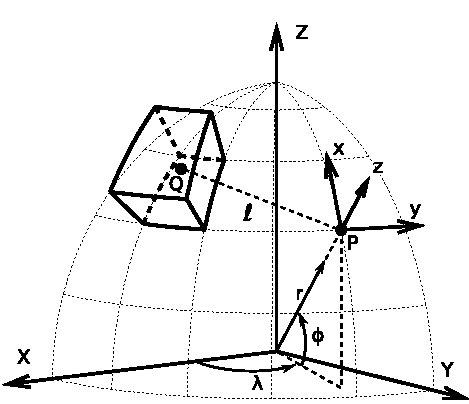
\includegraphics[width=0.9\linewidth]{figures/tesseroid-uieda.pdf}
\caption{
A spherical prism, also known as  Tesseroid, in a geocentric spherical coordinate system, with a computation point $P$ and its local north oriented Cartesian coordinate system. Picture made by \citep{Uieda2015}.
}
\label{fig:tesseroid-uieda}
\end{figure}

In order to develop a forward model that computes the gravity field generated by any tesseroid with arbitrary variable density, the Taylor series expansion is not well suited, because it would need to derive the series expansion terms for each density function. On the other hand, the GLQ allows us to calculate them for any density function without any other information but the function itself.

\citet{Uieda2016} developed a forward gravity model based on tesseroids with homogeneous densities using the GLQ approximation method.
It has been originally implemented in command line programs written in C programming language. Although, it has been ultimately ported to Python and included in the open-source library Fatiando a Terra \citep{Uieda2013} for geophysical modelling and inversion.

It's well known that the GLQ method becomes less accurate when the computation point is closer to the tesseroid \citep{Ku1977} or for smaller GLQ order. 
Although the model developed by \citet{Uieda2016} uses a second order GLQ, it ensures the accuracy implementing a modified version of the adaptive discretization of \citet{Li2011}.
It consist in splitting the tesseroid into smaller ones when a certain distance-size ratio ($D$) is greater than a predefined value that controls the precision of the computation.  \citet{Uieda2016} have also objectively obtained standard values of $D$ for gravity potential, gradients and tensor components comparing the fields generated by a spherical shell, which constitutes a special case of the volume integrals that has analytical solution \citep{LaFehr1991, Mikuska2006, Grombein2013}\todo{citar mas??}.
The modifications made by \citet{Uieda2016} to the original adaptive discretization method \citep{Li2011} consist in:
(1) a faster calculation of the distance from the computation point to the tesseroid and 
(2) the application of a stack based algorithm that speeds up the computation and gives more control over the recursion step.

We have enhanced the later implementation with a new forward gravity model that allows us to compute the gravity fields generated by any tesseroid with an arbitrary density function on any external point.
It's written in Python and Cython languages, obtaining an easy to use library that runs precompiled code for the more time consuming functions.

In order to ensure the accuracy of the numerical approximation, we have compared its results with a spherical shell with linear and exponential density functions, similar to the test performed by \cite{Uieda2016}. Although in this case, the analytical expressions for both density functions had to be derived.

It also makes use of some previously existing classes and functions from Fatiando a Terra, what saved us time and allowed us to focus on the new enhancements. Furthermore, we have the intention to include it into a future release of the Fatiando a Terra library in order to make its distribution and maintenance easier.

In the following sections we will describe how the new algorithm works, its theoretical background and obtain the distance-size ratio values needed to get a good accuracy in the computation.

%%%%%%%%%%%%%%%%%%%%%%%%%%%%%%%%%%%%%%%%%%%%%%%%%%%%%%%%%%%%%%%%%%%%%%%%%%%%%%

\section{Theory}

The spherical prisms known as tesseroids are mass elements defined in a geocentric spherical coordinate system bounded by a pair of parallels, a pair of  meridians, and two concentric spherical surfaces.
We define an external computation point $P(r, \phi, \lambda)$ where the gravity fields generated by the tesseroid are going to be calculated with respect to the local north oriented Cartesian coordinate system located at $P$.
In the special case of homogeneous density, the gravity potential, gradient and Marussi tensor components can be calculated through the integrals obtained by \citet{Grombein2013} \citep[see also][]{Uieda2016}.

In our case, we will suppose that the tesseroid has an arbitrary variable density in depth, this means that only depends on the radius spherical coordinate. Thus, the integrals for the gravity fields are slightly modified.

\begin{equation}
    V(r,\phi,\lambda) = G
    \int\limits_{\lambda_1}^{\lambda_2}
    \int\limits_{\phi_1}^{\phi_2}
    \int\limits_{r_1}^{r_2}
    \frac{\rho(r')}{\ell} \kappa \,  dr' d\phi' d\lambda',
\label{eq:tesseroid-pot}
\end{equation}
\begin{equation}
    g_{\alpha}(r,\phi,\lambda) = G
    \int\limits_{\lambda_1}^{\lambda_2}
    \int\limits_{\phi_1}^{\phi_2}
    \int\limits_{r_1}^{r_2}
    \rho(r') \frac{\Delta_\alpha}{\ell^3}
    \kappa \, dr' d\phi' d\lambda',
\label{eq:tesseroid-grav}
\end{equation}
\begin{equation}
    g_{\alpha\beta}(r,\phi,\lambda) = G
    \int\limits_{\lambda_1}^{\lambda_2}
    \int\limits_{\phi_1}^{\phi_2}
    \int\limits_{r_1}^{r_2}
    \rho(r') I_{\alpha\beta} \, \kappa \, dr' d\phi' d\lambda' ,
    \label{eq:tesseroid-tensor}
\end{equation}

\noindent where

\begin{equation}
    I_{\alpha\beta} =
    \left(
        \frac{3\Delta_{\alpha} \Delta_{\beta}}{\ell^5} -
        \frac{\delta_{\alpha\beta}}{\ell^3}
    \right) ,
    \label{eq:tesseroid-tensor-kernel}
\end{equation}

\noindent $\alpha, \beta \in \{x, y, z\}$,
$\rho(r')$ is the density function that depends on the radius coordinate,
$\delta_{\alpha\beta}$ is Kronecker's delta,
$G = 6.674\times10^{-11}\, \text{m$^3$kg$^{-1}$s$^{-1}$}$ is the gravitational constant and

\begin{equation}
    \Delta_x = r'[\cos\phi\sin\phi' - \sin\phi\cos\phi'
               \cos(\lambda' - \lambda)],
\end{equation}
\begin{equation}
    \Delta_y = r' \cos \phi' \sin(\lambda' - \lambda),
\end{equation}
\begin{equation}
    \Delta_z = r' \cos \psi - r,
\end{equation}
\begin{equation}
    \kappa = {r'}^2 \cos \phi',
\end{equation}
\begin{equation}
    \ell = \sqrt{{r'}^2 + r^2 - 2 r' r \cos \psi},
\label{eq:ell}
\end{equation}
\begin{equation}
    \cos\psi = \sin\phi\sin\phi' + \cos\phi\cos\phi'
                 \cos(\lambda' - \lambda).
\label{eq:cospsi}
\end{equation}


According to \citet[p.~390]{Hildebrand1987}, we can approximate any integral in the interval $[-1, 1]$ using a $N$th order GLQ, i.e. by a weighted sum of the integration kernel evaluated on the roots of the $N$th Legendre polynomial:

\begin{equation}
    \int\limits_{-1}^1 f(x) dx \approx \frac{b-a}{2} \sum_{i=1}^N W_i f(x_i),
\end{equation}

\noindent where $x_i$ are the roots of the $N$th Legendre polynomial $P_N(x)$ and $W_i$ are the weights of each term:

\begin{equation}
    W_i = \frac{2}{(1-x_i^2)[P_N^\prime(x_i)]^2},
\end{equation}

\begin{equation}
    P_N(x_i) = 0, \quad \forall i = {1,\dots,N}.
\end{equation}

In case of an integration defined on a arbitrary interval, e.g. $[a,b]$, we can scale the nodes and perform a similar approximation:

\begin{equation}
    \int\limits_a^b f(x) dx \approx \frac{b-a}{2} \sum_{i=1}^N W_i f(x_i^s),
\end{equation}

\noindent where $x_i^s$ is the scaled $x_i$ root in the $[a,b]$ interval, also called nodes of the quadrature:

\begin{equation}
    x_i^s = \frac{b-a}{2} x_i + \frac{b+a}{2}.
\end{equation}

For example, if we use a second order GLQ, the roots of the $P_2(x)$ Legendre polynomial and its corresponding weights are $x_i = \pm 0.577350269$ and $W_i = 1$, respectively.

Our intention is to use GLQ to approximate the volume integrals from equations \ref{eq:tesseroid-pot}-\ref{eq:tesseroid-tensor}. 
When tesseroids have variable densities, we can write the integral kernels as the product of a certain function $g$ and the density function:

\begin{equation}
    f(r', \phi', \lambda') = \rho(r') g(r', \phi', \lambda'),
\end{equation}

\noindent and then apply the quadrature to every integral corresponding to each spherical coordinate, obtaining a similar expression to the one shown by \citet{Asgharzadeh2007} and \citet{Uieda2016}:

\iftwocol{
\begin{equation}
    \begin{split}
        \iiint\limits_\Omega \rho(r') g(r', \phi', \lambda') 
        d\Omega \approx& \\
        A 
        \sum\limits_{i=1}^{N^r}
        \sum\limits_{j=1}^{N^\phi}
        \sum\limits_{k=1}^{N^\lambda}
        & W_i^r W_j^\phi W_k^\lambda \rho(r_i) g(r_i, \phi_j, \lambda_k),
    \end{split}
\label{eq:glq-var-dens}
\end{equation}
}{
\begin{equation}
    \iiint\limits_\Omega \rho(r') g(r', \phi', \lambda') d\Omega \approx
    A 
    \sum\limits_{i=1}^{N^r}
    \sum\limits_{j=1}^{N^\phi}
    \sum\limits_{k=1}^{N^\lambda}
    W_i^r W_j^\phi W_k^\lambda \rho(r_i) g(r_i, \phi_j, \lambda_k),
\label{eq:glq-var-dens}
\end{equation}
}

\noindent where

\begin{equation}
    A = 
    \frac{(\lambda_2 - \lambda_1)(\phi_2 - \phi_1)(r_2 - r_1)}{8}.
\end{equation}

From equation \ref{eq:glq-var-dens} we can observe that the GLQ approximates the gravity fields of a tesseroid with variable density as the ones generated by point masses located at the nodes of the Legendre polynomials.
Furthermore, the information of the density function is summarised as the values it assumes in those nodes.
Although this may sound discouraging, we intent to prove otherwise and show that this method, along with a well fitted discretization algorithm, approximates the gravity fields with good accuracy and precision.\todo{no se si poner esta ultima oracion}

%%%%%%%%%%%%%%%%%%%%%%%%%%%%%%%%%%%%%%%%%%%%%%%%%%%%%%%%%%%%%%%%%%%%%%%%%%%%%%

\subsection{Analytical Solutions for Spherical Shell}

In order to test the accuracy of the GLQ approximation, \citet{Uieda2016} and \citet{Grombein2013} have compared the computed gravity fields with the ones generated by a spherical shell, the exceptional case with analytical solution \citep{Mikuska2006,Grombein2013}.

In case of variable density tesseroids, the comparison must obviously be made with a variable density spherical shell, whose analytical solution will depend on the chosen density function.
Because the literature has not offered it yet, we needed to develop ourselves.

Lets consider a spherical shell with inner and outer radii $R_1$ and $R_2$, respectivetly, which density depends on the radius spherical coordinate (Figure \ref{fig:spherical-shell}).
The gravity potential generated by the shell on an arbitrary external point $Q(0,0,r)$ located along the $z$ axe at a distance $r$ can be written as follows:

\begin{figure}
\centering
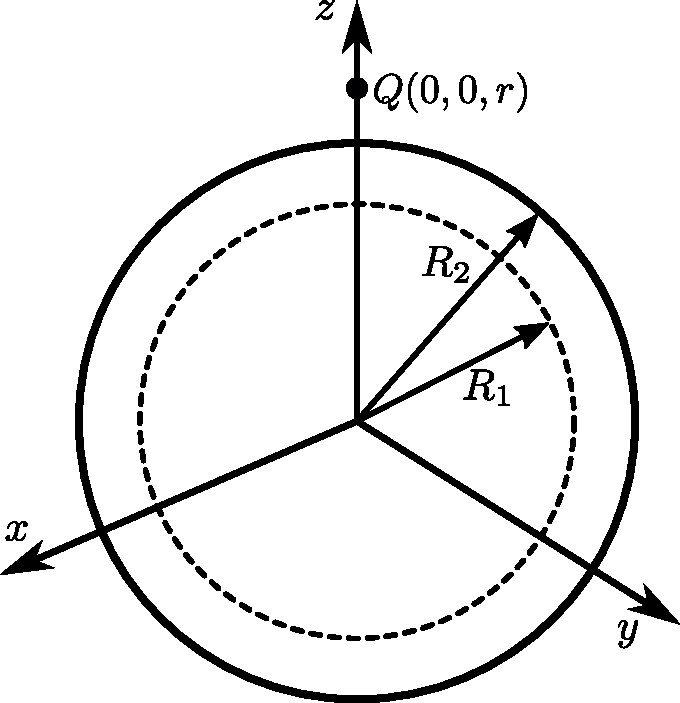
\includegraphics[width=0.9\linewidth]{figures/spherical-shell.pdf}
\caption{
Spherical shell with inner and outer radii $R_1$ and $R_2$, respectively.
The computation point $Q$ is located in the $z$ axe at a distance $r$ from the centre of the shell.
For practical purposes we will assume that $Q$ is outside the outer radii, i.e. $r > R_2$.
}
\label{fig:spherical-shell}
\end{figure}

\begin{equation}
    V_\text{sh}(r) = G 
    \int\limits_0^{2\pi}
    \int\limits_{-\frac{\pi}{2}}^\frac{\pi}{2}
    \int\limits_{R_1}^{R_2}
    \frac{\rho(r')}{\ell} {r'}^2 \cos\phi' \, 
    dr' d\phi' d\lambda',
\end{equation}

\noindent where $\ell$ is defined as in equation \ref{eq:ell}.
The computation point $Q$ is located at latitude $\phi=90^\circ$, so $\ell$ and $\cos\psi$ (defined in equation \ref{eq:cospsi}) get simplified:

\begin{equation}
    \cos\psi = \sin\phi', \quad
    \ell = \sqrt{r'^2 + 2 r r' \sin\phi' + r^2}.
\end{equation}

Due to the rotational symmetry along the $z$ axe, the integration in $\lambda'$ is straightforward:

\begin{equation}
    V_\text{sh}(r) = 2\pi G 
    \int\limits_{-\frac{\pi}{2}}^\frac{\pi}{2}
    \int\limits_{R_1}^{R_2}
    \frac{\rho(r') {r'}^2 \cos\phi'}{\sqrt{r'^2 + 2 r r' \sin\phi' + r^2}}
    \, dr' d\phi',
\end{equation}

\noindent and the integration in $\phi'$ can be performed independently of the density function.
Using \citet{sagemath} we obtain the following expression:

\iftwocol{
\begin{equation}
    \begin{split}
        V_\text{sh}(r) = 2\pi G
        \int\limits_{R_1}^{R_2}
        \Big[ & \sqrt{r^2 + r'^2 + 2rr'} - \\
        & \sqrt{r^2 + r'^2 - 2rr'}
        \Big] \frac{r'\rho(r')}{r} \, dr'.
    \end{split}
\label{eq:shell-pot-sqrts}
\end{equation}
}{
\begin{equation}
    V_\text{sh}(r) = 2\pi G
    \int\limits_{R_1}^{R_2}
    \Big[ \sqrt{r^2 + r'^2 + 2rr'}  -
    \sqrt{r^2 + r'^2 - 2rr'} 
    \Big] \frac{r'\rho(r')}{r} \, dr'.
\label{eq:shell-pot-sqrts}
\end{equation}
}

For our purposes we can assume that the computation point $Q$ is outside the outer radii, i.e. $r>R_2$ ($R_2 \geq r'$), and simplify the square roots in equation \ref{eq:shell-pot-sqrts}:

\begin{equation}
    \sqrt{r^2 + r'^2 + 2rr'} = |r + r'| = r + r',
\end{equation}
\begin{equation}
    \sqrt{r^2 + r'^2 - 2rr'} = |r - r'| = r - r',
\end{equation}

\noindent what leads to the following expression of the potential of the spherical shell:

\begin{equation}
    V_\text{sh}(r) = \frac{4\pi G}{r}
    \int\limits_{R_1}^{R_2} {r'}^2 \rho(r') \, dr'.
\label{eq:shell-pot}
\end{equation}

The equation \ref{eq:shell-pot} allows to easily obtain the exact gravity field generated by a spherical shell with a variable density in depth on any outside point located in the $z$ axe.
Due to the rotational symmetry along any axe that passes through the centre of the shell, the potential in equation \ref{eq:shell-pot} reassembles the gravity field on any outside point at distance $r$ from the its centre.

For any density $\rho(r')$, the gradient and Marussi tensor components can be obtained as \citet{Grombein2013} does. Only the vertical gradient component ($g_z$) and the diagonal Marussi tensor components ($g_{xx}$, $g_{yy}$, $g_{zz}$) are not zero, and can be easily determined from the potential $V_\text{sh}$:

\begin{equation}
    g_z = \frac{V_\text{sh}(r)}{r},
\end{equation}
\begin{equation}
    g_{xx} = g_{yy} = -\frac{V_\text{sh}(r)}{r^2}, \quad
    g_{zz} = \frac{2V_\text{sh}(r)}{r^2}.
\end{equation}

For practical purposes we are going to obtain the gravity potential for two very different functions in the perspective of they variation in $r'$: a linear density and an exponential density.


\subsubsection{Linear Density}

If the density of the spherical shell is a linear function in the radius coordinate, i.e.:

\begin{equation}
    \rho(r') = ar' + b,
\end{equation}

\noindent then the gravity potential generated on any computation point at distance $r$ from its centre can be obtained from the following expression:

\begin{equation}
    V_\text{sh}^\text{lin}(r) = \pi G \left[ 
    a \frac{R_2^4 - R_1^4}{r} +
    b \,\frac{4}{3} \frac{R_2^3 - R_1^3}{r} \right].
    \label{eq:shell-pot-linear}
\end{equation}

The second term on equation \ref{eq:shell-pot-linear} reassembles the potential generated by a spherical shell with homogeneous density $\rho = b$ \citep{Mikuska2006,Grombein2013}.
So, this potential can be read as the combination of a spherical shell with the later homogeneous density and the same shell with variable density $\rho(r') = ar'$.


\subsubsection{Exponential Density}

If, on the other hand, the spherical shell has an exponential density in the radius coordinate,

\begin{equation}
    \rho(r') = Ae^{-(r' - \Delta h)/b},
\end{equation}

\noindent the potential can be written as follows:

\iftwocol{
\begin{equation}
    \begin{split}
        V_\text{sh}^\text{exp}(r) = \frac{4\pi G}{r} 
        Ab \, e^\frac{\Delta h}{b}
        \Big[
        & (R_1^2 + 2R_1 b + 2b^2)e^{-\frac{R_1}{b}} - \\
        & (R_2^2 + 2R_2 b + 2b^2)e^{-\frac{R_2}{b}}
        \Big].
    \end{split}
\label{eq:shell-pot-exp}
\end{equation}
}{
\begin{equation}
    V_\text{sh}^\text{exp}(r) = \frac{4\pi G}{r} 
    Ab \, e^\frac{\Delta h}{b}
    \Big[
    & (R_1^2 + 2R_1 b + 2b^2)e^{-\frac{R_1}{b}} - \\
    & (R_2^2 + 2R_2 b + 2b^2)e^{-\frac{R_2}{b}}
    \Big].
\label{eq:shell-pot-exp}
\end{equation}
}

%%%%%%%%%%%%%%%%%%%%%%%%%%%%%%%%%%%%%%%%%%%%%%%%%%%%%%%%%%%%%%%%%%%%%%%%%%%%%%%

\section{Implementation}

We have developed a Python library that computes the gravity fields generated by any Tesseroid with variable density in depth through the GLQ to numerically approximate the volume integrals. It's freely available under the BSD 3-clause open-source library and can be downloaded from the following repository: \todo{agregar repo, vale la pena poner el link?}

Although it's a Python library, the core functions of the computation are written in Cython, a superset of Python language that allows us generate efficient C code through the Cython compiler.
This produces a precompiled library whose functions and classes can be called from regular Python code, what allowed us to make it compatible with the preexisting open-source library Fatiando a Terra \citep{Uieda2013}.

Its usage is very similar to the code for homogeneous tesseroid already in Fatiando a Terra (version 0.5):

\begin{enumerate}
\renewcommand{\theenumi}{(\arabic{enumi})}
\item Define a single tesseroid (or a tesseroid mesh) with the Fatiando a Terra classes.
\item Add a predefined Python density function to the tesseroid (or each tesseroid in the mesh).
\item Calculate the desired gravity field (potential, gradient or tensor component) in any set of computation points with our new functions.
\end{enumerate}

The existing code in Fatiando a Terra (v.~0.5) for homogeneous tesseroid is optimised through the Numba compiler.
Due to difficulties when passing a Python function as argument of precompiled Numba methods, we have decided to rewrite them in Cython language, keeping the homogeneous tesseroid calculation and adding the new variable density code.

\todo{speed comparison between homogeneous and variable density}

From equation \ref{eq:glq-var-dens} we saw that the GLQ approximates the volume integrals as the gravitational effect of $N_\lambda N_\phi N_r$ point masses, where $N_i$ are the orders of the quadrature for the integral on each coordinate, with $i \in \{ \lambda, \phi, r \}$.

If we set the GLQ orders to fixed values, it's easy to conclude that the nearer the computation point is to the tesseroid, the accuracy of the approximation is reduced and the point masses effect becomes more noticeable than the tesseroid we want to approximate.
A more complete analysis of this conclusion can be found in \citet{Ku1977, Li2011, Uieda2016}.

Instead of increasing the GLQ orders, what leads to a more time consuming computation, adaptive discretization algorithms have been applied in previous works \citep{Li2011, Uieda2016}.
They basically consist in dividing the tesseroid based on a ratio between its size and the distance between its geometric centre and the computation point.

In order to make the computation more efficient, we use only second order GLQ for each integration, and we ensure the accuracy of the method through the application of the modified adaptive discretization algorithm developed by \citet{Uieda2016}.

Given an arbitrary tesseroid, \citet{Uieda2016} redefined its dimensions: $L_\lambda$, $L_\phi$ and $L_r$, where the former ones are the arc-distances measured along its top surface and $L_r$ is the difference between the radii of the top and bottom surfaces.
We must check that the following inequality is satisfied:

\begin{equation}
\frac{d}{L_i} \geq D,
\label{eq:distance-size-ratio}
\end{equation}

\noindent where $i \in \{\lambda, \phi, r\}$, $d$ is the distance between the geometric centre of the tesseroid and the computation point and $D$ is a predefined value called distance-size ratio.
If the inequality \ref{eq:distance-size-ratio} is not held for any spherical coordinate, then the tesseroid must be divided by half in that direction.
A more complete description of the modified adaptive discretization algorithm can be found in \citet{Uieda2016}.

In this way, the numerical approximation efficiently improves its accuracy and
gives the user more control over the computation by allowing to stop the division of the tesseroids when their dimensions are lower than a certain value (e.g. less than 10cm).

On the other hand, the accuracy is exclusively controlled by the value assigned to the distance-size ratio $D$, which cannot be easily related to the error of the approximation.
In order to solve this, \citet{Uieda2016} compared the numerical computation with the analytical solution for a spherical shell with homogeneous density.

We have performed similar tests, but now with variable density spherical shell. From the infinite density functions that can be proposed, we have chosen two characteristic ones: a linear and an exponential functions.
The first one represents the simpler variation, while the second one symbolise the fastest varying function.
The analytical solutions for these two types of functions were previously obtained and shown in equations \ref{eq:shell-pot-linear} and \ref{eq:shell-pot-exp}.


%%%%%%%%%%%%%%%%%%%%%%%%%%%%%%%%%%%%%%%%%%%%%%%%%%%%%%%%%%%%%%%%%%%%%%%%%%%%%%%

\section{Acknowledgments}

We are indebted to the developers and maintainers of the open-source
software without which this work would not have been possible.

%%%%%%%%%%%%%%%%%%%%%%%%%%%%%%%%%%%%%%%%%%%%%%%%%%%%%%%%%%%%%%%%%%%%%%%%%%%%%%%

\bibliographystyle{gji}
\bibliography{bibtex/references}

\end{document}
